\section{Playing with projections and transformations}

I like to start with a simple basefunction, and then distort it.

Nice basefunctions:
\begin{itemize}
    \item simple geometric
    \item recursive
\end{itemize}

Nice distortions: 
\begin{itemize}
    \item sinusoidal (Fourier: add overtones)
    \item imaginary (Laplace: add more dimensions)
    \item stepfunction (Mandelbrot: cut off some of them)
    \item flat onto spherical (Mapprojection)
    \item circle rolled around circle (Spirograph)
    \item Copy and rotate
    \item shadows
\end{itemize}

Finally, we can refine the result. 
\begin{itemize}
    \item change paras over time
    \item heatmap
    \item path
\end{itemize}

We will try an example now. Take a simple geometric shape. Create it's fourier representation. Add some overtones to it. Convert it back into geometric space. What do you get?

There are basically two ways we can achive this. The first is using ordinary (that is, one-dimenstional) Fourier and parametrised shapes: 
\begin{itemize}
    \item a1: Take some parameterised Shape in $\reals^3$: $S(f(t))$
    \item a2: Extract $f(t)$
    \item a3: Express $f(t)$ in its Fourier representation: $f(t) = \sum \alpha_i b_i$, where $b_i$ is one-dimensional
    \item a4: add some overtones to obtain $f'(t)$
    \item a5: Obtain $S'$ as $S(f'(t))$ 
\end{itemize}

The second approach seems simpler, but requires tree dimensional Fourier: 
\begin{itemize}
    \item b1 (= a2): Take a shape $S(\vec{v})$
    \item b2 (= a3): $S(\vec{v}) = \sum \alpha_i \vec{b}_i$
    \item b3 (= a4, a5): Obtain $S'$ by adding overtones to $S$
\end{itemize}






\section{Fourier on sound and geometric objects}

\subsection{Basics: Fourier in one dimension}

\subsubsection{Representing a function under a Fourier base}

 The Fourier functions $\{sin(nt), cos(nt) | n \in \naturals \}$ form an orthogonal base for all functions in the space of square-integrable functions that are periodic between $-\pi$ and $\pi$. Lets first get some familiarity with Fourier analysis.

At first we'll try to express a simple function in a fourier base: 
$$ f(t) = sin(t) = \alpha_0 + \sum_n^\infty \alpha_n cos(n t)  + \sum_n^\infty \beta_n sin(n t)$$

It's comparatively easy to calculate the coefficients of this series\footnote{The term $\frac{1}{\pi}$ is not strictly neccessary for an orthogonal base, but it is very convenient, since it makes our base ortho\emph{normal}.}: 

$$ \alpha_0 = \frac{1}{\pi} \int_{-\pi}^\pi sin(t) \diff{t} = 0$$
$$ \alpha_1 = \frac{1}{\pi} \int_{-\pi}^\pi sin(t) cos(t) \diff{t} = 0$$
$$ \alpha_2 = .. = 0 $$
$$ \alpha_3 = ... = 0 $$

$$ \beta_1 = \frac{1}{\pi} \int_{-\pi}^\pi sin(t) sin(t) \diff{t} = 1 $$
$$ \beta_2 = \frac{1}{\pi} \int_{-\pi}^\pi sin(t) sin(2t) \diff{t} = 0 $$
$$ \beta_3 = ... = 0 $$ 

In other words: the only amplitude different from $0$ is $\beta_1 = 1$

We'll be using python for our Fourier-analysis, where it is more common to work with the exponential/imaginary representation of the Fourier functions. This representation is based on Eulers formula: 

$$ e^{it} = \cos(t) + i\sin(t)$$

Using this equation we can rewrite the Fourier base as $\{e^{int} | n \in \naturals \}$.
 Using this base we get as the only nonzero coefficient: 
 $$ \gamma_1 = \frac{1}{\pi} \int_{-\pi}^\pi sin(t) e^{it} \diff{t} = i $$

Having imaginary amplitudes may be intimidating at first, but really it's very simple. The real part of such an amplitude equals the amplitude of the equivalent $\cos$ term, whereas the imaginary part equals the amplitude of the $\sin$ term. 

\subsubsection{Bringing in arbitrary intervals}

In the previous section, when we wrote the index $n$, we meant that the function would repeat itself $n$ times within the interval $[-\pi, \pi]$ - it has a frequency of $f_n = \frac{n}{2\pi}$.

However, in reality we will deal with functions that are periodic over an unspecified interval $[-T,T]$ \footnote{In \emph{real} reality, we will not deal with periodic functions at all. But more on that later}. To acomodate this, we can expand our notion of Fourier basis to the space of all square integrable functions that are periodic between $[-T, T]$. Our base now consists of $\{sin(\frac{2 \pi n}{T} t), cos(\frac{2 \pi n}{T} t) | n \in \naturals \}$ or $\{ e^{i \frac{2 \pi n}{T} t} | n \in \naturals \}$.

Lets consider the function $f(t) = \sin(\frac{2\pi}{T}t)$. Just like before, it's easy to calculate this functions Fourier coefficients, and just like before, only one of them is nonzero: 

$$ \gamma_1 = \frac{1}{T} \int_{-T}^T \sin(\frac{2\pi}{T} t) e^{i \frac{2 \pi}{T} t} \diff{t} = i$$

The frequency that goes associated with the index $n=1$ is $f_n = \frac{n}{T} = 0.1$. 

\subsubsection{Implementation and verification in python}

It's time to get our hands dirty and learn about python's implementation of Fourier transforms. We'll try to use pythons \inlinecode{fft} library to recreate the previous section: 

\begin{lstlisting}
import numpy as np
import matplotlib.pyplot as plt

delta = 0.01
T = 10
t = np.arange(-T, T, delta)
data = np.sin(2 * np.pi * t / T)
amps = np.fft.fft(data)
frqs = np.fft.fftfreq(data.size, delta)

f, (ax1, ax2) = plt.subplots(1, 2)
ax1.plot(frqs, np.real(amps))
ax2.plot(frqs, np.imag(amps))
plt.show()
\end{lstlisting}

As expected, the plot shows a high amplitude at the frequency 0.1. Not quite as expected is the other peak at frequency -0.1. What's up with that? In fact, there are a few phenomena that warrant further explanation: 

\begin{itemize}
    \item Amplitudes are not really 0 where they should be, they only are very close to 0. This is merely an artifact of numerical computation that we won't bother with any further. 
    \item The amplitudes are not normalized to $T$. This, too, should not pose any difficulties for us, as we will not be using the concrete values of the amplitudes in this project. 
    \item How does fft chose which frequencies to consider? Here, for some reason, it's between -50 and 50.
    \item Why are there positive and negative frequencies?
    \item For now, we have chosen \inlinecode{t} to cover the interval $[-T, T]$ perfectly. But what if we have \inlinecode{t} too long or too short? Surprisingly, this doesn't seem to change the estimated frequencies very much. 
\end{itemize}


\subsubsection{Our first frequency domain operations: adding overtones}

We went trough all the trouble of representing $f(t)$ over a Fourier base for a reason: there are operations that are natural in the frequency domain that don't exactly come easily in time domain. One of those operations would be adding overtones. 


\begin{lstlisting}[language=python]
import numpy as np
import matplotlib.pyplot as plt
import simpleaudio as sa


sampleRate = 44100


def addXHalfTonesTo(basefreq, steps):
    return basefreq * (2 ** (steps / 12.0))


def play(data, sampleRate):
    dataNrm = data * 32767 / np.max( np.abs( data ))
    data16 = dataNrm.astype(np.int16)
    return sa.play_buffer(data16, 1, 2, sampleRate)



# creating the data
delta = 1.0 / sampleRate
T = 1
t = np.arange(0, T, delta)
data = np.sin( t * 440 * 2 * np.pi )
#play(data, sampleRate)


# transform to frequency domain
amps = np.fft.fft(data)
frqs = np.fft.fftfreq(data.size, delta)

# filter out the less important frqs
# add chord on top of basetone
thrsh = 0.1 * np.max(np.abs(amps))
ampsNew = np.zeros(np.shape(amps), dtype=np.complex128)
for i, a in enumerate(amps):
    if np.abs(a) > thrsh:
        f1 = frqs[i]
        f2 = np.round(addXHalfTonesTo(f1, 4))
        f3 = np.round(addXHalfTonesTo(f1, 7))
        i2 = np.where(frqs == f2)[0]
        i3 = np.where(frqs == f3)[0]
        ampsNew[i] += a
        ampsNew[i2] += a
        ampsNew[i3] += a

# convert back to timedomain
dataNew = np.fft.ifft(ampsNew)
play(dataNew, sampleRate)


# plot
f, ((ax1, ax2), (ax3, ax4)) = plt.subplots(2, 2)
ax1.plot(t, data)
ax2.plot(frqs, np.abs(amps))
ax3.plot(t, dataNew)
ax4.plot(frqs, np.abs(ampsNew))
plt.show()
\end{lstlisting}


\subsubsection{Windowing}
Now, in reality we will not be dealing with a allways constant sinewave. A piece of music is composed of different tones at different times. If we don't account for that, we get something like this: 

\begin{lstlisting}[language=python]
import numpy as np
import matplotlib.pyplot as plt
import simpleaudio as sa


sampleRate = 44100


def addXHalfTonesTo(basefreq, steps):
    return basefreq * (2 ** (steps / 12.0))


def play(data, sampleRate):
    dataNrm = data * 32767 / np.max( np.abs( data ))
    data16 = dataNrm.astype(np.int16)
    return sa.play_buffer(data16, 1, 2, sampleRate)



# creating the data
delta = 1.0 / sampleRate
T = 1
t = np.arange(0, T, delta)
fa = 440
fc = addXHalfTonesTo(fa, 4)
fd = addXHalfTonesTo(fc, 3)
a = np.sin( t * fa * 2 * np.pi )
c = np.sin( t * fc * 2 * np.pi )
d = np.sin( t * fd * 2 * np.pi )
t = np.concatenate((t, t, t, t))
data = np.concatenate((a, c, d, c))
#play(data, sampleRate)


# transform to frequency domain
amps = np.fft.fft(data)
frqs = np.fft.fftfreq(data.size, delta)

# filter out the less important frqs
# add chord on top of basetone
thrsh = 0.1 * np.max(np.abs(amps))
ampsNew = np.zeros(np.shape(amps), dtype=np.complex128)
for i, a in enumerate(amps):
    if np.abs(a) > thrsh:
        f1 = frqs[i]
        f2 = np.round(addXHalfTonesTo(f1, 4))
        f3 = np.round(addXHalfTonesTo(f1, 7))
        i2 = np.where(frqs == f2)[0]
        i3 = np.where(frqs == f3)[0]
        ampsNew[i] += a
        ampsNew[i2] += a
        ampsNew[i3] += a

# convert back to timedomain
dataNew = np.fft.ifft(ampsNew)
play(dataNew, sampleRate)


# plot
f, ((ax1, ax2), (ax3, ax4)) = plt.subplots(2, 2)
ax1.plot(t, data)
ax2.plot(frqs, np.abs(amps))
ax3.plot(t, dataNew)
ax4.plot(frqs, np.abs(ampsNew))
plt.show()

\end{lstlisting}


Thats why we use windowing. Windowing is the process of cutting an incomming signal in small chunks, for wich we create an individual Fourier analysis. This way, at tone c, we don't have to drag along tone a any more; a has long been forgotten by the analysis. 



\begin{lstlisting}[language=python]
import numpy as np
import matplotlib.pyplot as plt
import simpleaudio as sa


sampleRate = 44100


def first(data, cond):
    for i, d in enumerate(data):
        if cond(d):
            return i, d


def addXHalfTonesTo(basefreq, steps):
    return basefreq * (2 ** (steps / 12.0))


def overtone(steps, frqs, amps):
    ampsNew = np.zeros(np.shape(amps), dtype=np.complex128)
    for i, a in enumerate(amps):
        if np.abs(a) > 0: 
            f1 = frqs[i]
            f2 = np.round(addXHalfTonesTo(f1, steps))
            i2 = np.where(frqs == f2)
            #ampsNew[i] += a
            ampsNew[i2] += a
    return ampsNew
            

def play(data, sampleRate):
    dataNrm = data * 32767 / np.max( np.abs( data ))
    data16 = dataNrm.astype(np.int16)
    po = sa.play_buffer(data16, 1, 2, sampleRate)
    po.wait_done()
    return po


def filterLower(amps, perc):
    thrsh = perc * np.max( np.abs( amps ))
    ampsNew = np.zeros(np.shape(amps), dtype=np.complex128)
    for i, a in enumerate(amps):
        if np.abs(a) > thrsh: 
            ampsNew[i] = a
    return ampsNew


def distort(frqs, amps):
    ampsFiltered = filterLower(amps, 0.5)
    terz = overtone(4,frqs, ampsFiltered)
    quint = overtone(7, frqs, ampsFiltered)
    return ampsFiltered + terz + quint


def autotune(frqs, amps):
    ampsFiltered = filterLower(amps, 0.9999)
    ampsTuned = np.zeros( np.shape( ampsFiltered), dtype=np.complex128 )
    halfToneFreqs = [addXHalfTonesTo(220, x) for x in range(23)]
    for i, a in enumerate(ampsFiltered):
        if np.abs(a) > 0: 
            f = frqs[i]
            if f > 0:
                ihh, fhh = first(halfToneFreqs, lambda fc: fc >= f)
                fhl = halfToneFreqs[ihh-1]
                disth = np.abs(fhh - f)
                distl = np.abs(fhl - f)
                fh = fhl if distl < disth else fhh
                inew, fnew = first(frqs, lambda fc: fc >= fh)
                ampsTuned[inew] = a
    return ampsTuned
        

def chunks(data, length):
    C = int( np.ceil( len(data) / length ))
    chunks = []
    start = 0
    end = length
    for c in range(C):
        chunks.append(data[start:end])
        start += length
        end += length
    return chunks


delta = 1.0 / sampleRate
t = np.arange(0, 2, delta)
freq = lambda t: 220 + 220 * t / 2
data = np.sin(t * freq(t) * 2 * np.pi)

origAmps = []
tunedAmps = []
tunedChunks = []
chunksize = int(data.size / 4)
for chunk in chunks(data, chunksize):
    frqs = np.fft.fftfreq(chunk.size, delta)
    amps = np.fft.fft(chunk)
    ampsNew = autotune(frqs, amps)
    dataNew = np.fft.ifft(ampsNew)
    origAmps.append(amps)
    tunedAmps.append(ampsNew)
    tunedChunks.append(dataNew)


dataNew = np.concatenate(tunedChunks)
play(data, sampleRate)
play(dataNew, sampleRate)


start = 0
stop = 700
f, axes = plt.subplots(4)
for i in range(4):
    axes[i].plot(frqs[start:stop], np.abs(origAmps[i][start:stop]))
    axes[i].plot(frqs[start:stop], np.abs(tunedAmps[i][start:stop]), 'r')
plt.show()

\end{lstlisting}

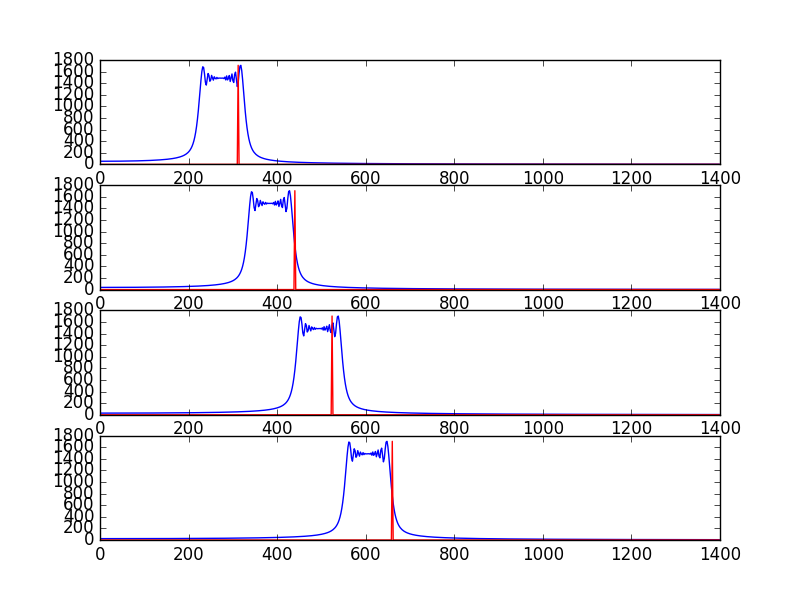
\includegraphics[width=0.7\textwidth]{images/autotune.png}


\subsection{Fourier in more than one dimensions}

\subsubsection{Mutliple input parameters}
Consider a simple black and white image. We'll describe the value at any pixel as $v(x, y)$, that is, $v: \reals^2 \to \reals$. Again, the base of the space of $(\reals^2 \to \reals)$ functions must consist of functions that are themselves $(\reals^2 \to \reals)$. The Fourier-representation of an image can be quite naturally obtained by: 


$$ v(x, y) = \sum_n^\infty \sum_m^\infty \alpha_{n,m} b_{n,m}(x, y) $$

where $b_{n,m}(x, y) = e^{i( \frac{n 2 \pi}{b_x - a_x} x + \frac{m 2 \pi}{b_y - a_y} y)}$ and  

$$ \alpha_{n,m} = \int_{a_x}^{b_x} \int_{a_y}^{b_y} v(x, y) e^{i( \frac{n 2 \pi}{b_x - a_x} x + \frac{m 2 \pi}{b_y - a_y} y)} \diff{y} \diff{x}$$

Generally, when a function takes two parameters, here $x,y$, then we also need two frequency parameters, here $n,m$. Analogously, for functions of three parameters we'd need three frequency parameters.


\subsubsection{Multiple output parameters: Vector valued functions}
In the previous section, we dealt with the space of functions mapping $\reals^2 \to \reals$. How about vector valued functions? Finally, we have arrived at the top level of abstraction when it comes to Fourier representations: the space of functions mapping $\reals^a \to \reals^b$. 

For example, consider the surface $\{ \vec{v} | v_z = v_x^2 + 3 v_y \}$. The set-expression can be rewritten into a function-expression: 

$$\vec{v}(x,y) = 
\begin{bmatrix} 
x \\
y \\
x^2 + 3 y
\end{bmatrix}$$

Here, we have an equation with two parameters ($v_x$ and $v_y$) mapping onto a 3d-vector $\vec{v}$. Consequently, the Fourier base of the space of surfaces, too, must consist of funcitons mapping $\reals^2 \to \reals^3$. 

As another example, consider an ellipsoid $\{\vec{v} | \frac{x^2}{r_1^2} + \frac{z^2}{r_2^2} + \frac{z^2}{r_3^2} = 1 \}$. This body can be parameterized as: 

$$ \begin{bmatrix}
x \\
y \\
z
\end{bmatrix} = 
\begin{bmatrix}
r_1 \cos{\theta} \cos{\phi} \\
r_2 \cos{\theta} \sin{\phi} \\
r_3 \sin{\theta}
\end{bmatrix} $$

This means we can represent the ellipsoid function as a sum of Fourier-base functions that map $[0\degree, 360\degree]^2 \to \reals^3$.

In general, we can represent any function mapping $\reals^a \to \reals^b$ by a Fourier base of functions from the same space. As for geometric bodies: as long as we can find a parameterisation of the body (that is continuous and sqare-integrable), we can also find a Fourier-representation\footnote{We cannot find a Fourier-representation of non-parameterisable sets. The reason for this is that sets don't form an inner-product space - or at least not without some whacky definitions.}. 

Surprisingly, this works just the same. Consider the ellipsoid in its parameterized representation: 

$$ \vec{v}(\phi, \theta) = 
\begin{bmatrix} 
    r_x \cos{\phi} \cos{\theta} \\
    r_y \cos{\phi} \sin{\theta} \\
    r_z \sin{\phi}
\end{bmatrix}  $$

$\vec{v}(\phi, \theta)$ is a member of the space $S = \{f: \reals^2 \to \reals^3\}$, so the basis must consist of functions of the same shape. Let's call one of the members of the basis $\vec{b}_{n,m}$. It must have the following structure: 

$$
\vec{b}_{n,m}(\phi, \theta) = 
\begin{bmatrix}
    b_{n,m}^x(\phi, \theta) \\
    b_{n,m}^y(\phi, \theta) \\
    b_{n,m}^z(\phi, \theta)
\end{bmatrix}
$$

Then the coefficient $\alpha_{n,m}$ is calculated like this: 

$$ \alpha_{n,m} = \int_{a_\theta}^{b_\theta} \int_{a_\phi}^{b_\phi} \vec{v}(\phi, \theta) \vec{b}_{n,m}(\phi, \theta) \diff{\phi} \diff{\theta} $$

$$ = \int_{a_\theta}^{b_\theta} \int_{a_\phi}^{b_\phi} (\vec{i} v^x(\phi, \theta) + \vec{j} v^y(\phi, \theta) \vec{k} v^z(\phi, \theta)) (\vec{i} b_{n,m}^x(\phi, \theta) + \vec{j} b_{n,m}^y(\phi, \theta) \vec{k} b_{n,m}^z(\phi, \theta)) \diff{\phi} \diff{\theta} $$

$$ = \int_{a_\theta}^{b_\theta} \int_{a_\phi}^{b_\phi} 1 v^x(\phi, \theta) b_{n,m}^x(\phi, \theta) + 0 + 0 + 0 + 1 v^y(\phi, \theta) b_{n,m}^y(\phi, \theta) + 0 + 0 + 0 + v^z(\phi, \theta) b_{n,m}^z(\phi, \theta) \diff{\phi} \diff{\theta} $$

$$ = \int_{a_\theta}^{b_\theta} \int_{a_\phi}^{b_\phi} v^x(\phi, \theta) b_{n,m}^x(\phi, \theta) \diff{\phi} \diff{\theta} + 
    \int_{a_\theta}^{b_\theta} \int_{a_\phi}^{b_\phi} v^y(\phi, \theta) b_{n,m}^y(\phi, \theta) \diff{\phi} \diff{\theta} + 
    \int_{a_\theta}^{b_\theta} \int_{a_\phi}^{b_\phi} v^z(\phi, \theta) b_{n,m}^z(\phi, \theta) \diff{\phi} \diff{\theta}  
$$

Let's apply the Fourier base $
\begin{bmatrix}
    b_{n,m}^x(\phi, \theta) \\
    b_{n,m}^y(\phi, \theta) \\
    b_{n,m}^z(\phi, \theta)
\end{bmatrix}
=
\begin{bmatrix}
    e^{i(\frac{n 2 \pi}{b_\phi - a_\phi}\phi + \frac{m 2 \pi}{b_\theta - a_\theta} \theta)} \\
    e^{i(\frac{n 2 \pi}{b_\phi - a_\phi}\phi + \frac{m 2 \pi}{b_\theta - a_\theta} \theta)} \\
    e^{i(\frac{n 2 \pi}{b_\phi - a_\phi}\phi + \frac{m 2 \pi}{b_\theta - a_\theta} \theta)} 
\end{bmatrix}
$ and the ellipsoid formula to this general expression. Then we get: 

$$ \alpha_{n,m} =   \int_{a_\theta}^{b_\theta} \int_{a_\phi}^{b_\phi} r_x \cos{\phi} \cos{\theta} e^{i(\frac{n 2 \pi}{b_\phi - a_\phi}\phi + \frac{m 2 \pi}{b_\theta - a_\theta} \theta)} \diff{\phi} \diff{\theta} + \\
                    \int_{a_\theta}^{b_\theta} \int_{a_\phi}^{b_\phi} r_y \cos{\phi} \sin{\theta} e^{i(\frac{n 2 \pi}{b_\phi - a_\phi}\phi + \frac{m 2 \pi}{b_\theta - a_\theta} \theta)} \diff{\phi} \diff{\theta} + \\
                    \int_{a_\theta}^{b_\theta} \int_{a_\phi}^{b_\phi} r_z \sin{\phi}              e^{i(\frac{n 2 \pi}{b_\phi - a_\phi}\phi + \frac{m 2 \pi}{b_\theta - a_\theta} \theta)} \diff{\phi} \diff{\theta}   $$
                
$$ \alpha_{n,m} =   r_x \int_{0}^{2\pi} \int_{0}^{2\pi} \cos{\phi} \cos{\theta} e^{i(n\phi + m\theta)} \diff{\phi} \diff{\theta} + \\
                    r_y \int_{0}^{2\pi} \int_{0}^{2\pi} \cos{\phi} \sin{\theta} e^{i(n\phi + m\theta)} \diff{\phi} \diff{\theta} + \\
                    t_z \int_{0}^{2\pi} \int_{0}^{2\pi} \sin{\phi}              e^{i(n\phi + m\theta)} \diff{\phi} \diff{\theta}   $$
                    
                    
Integrating yields:

...

Of course, the whole point is to graph the thing: 

\begin{lstlisting}[language=python]
import numpy as np

def ellipsoid(theta, phi, rx, ry, rz):
    x = rx * np.cos(theta) * np.cos(phi)
    y = ry * np.cos(theta) * np.sin(phi)
    z = rz * np.sin(theta)
    return x, y, z


def filterAmps(data, perc=0.8):
    dataAbs = np.abs(data)
    x, y = np.shape(data)
    thrsh = perc * np.max(dataAbs)
    filtered = np.zeros((x,y), dtype=np.complex128)
    for c in range(x):
        for r in range(y):
            if dataAbs[c,r] >= thrsh:
                filtered[c,r] = data[c,r]
    return filtered


def addOvertones(amps):
    x, y = np.shape(amps)
    ampsNew = np.zeros( (x, y), dtype=np.complex128 )
    for c in range(x): 
        for r in range(y):
            if np.abs(amps[c,r]) > 0:
                c2 = 2*c if 2*c < x else int(c/2)
                r2 = 2*r if 2*r < y else int(r/2)
                ampsNew[c,r] += amps[c,r]
                ampsNew[c,r2] += amps[c,r]
                ampsNew[c2,r] += amps[c,r]
                ampsNew[c2,r2] += amps[c,r]
    return ampsNew


rx = ry = rz = 1

data = np.zeros((360, 360, 3), dtype=np.float)
for t in np.arange(0,360):
    for p in np.arange(0, 360):
        data[t, p] = ellipsoid(t, p, rx, ry, rz)


ampsx = np.fft.rfft2(data[:,:,0])
ampsy = np.fft.rfft2(data[:,:,1])
ampsz = np.fft.rfft2(data[:,:,2])

ampsxF = filterAmps(ampsx, 0.001)
ampsyF = filterAmps(ampsy, 0.001)
ampszF = filterAmps(ampsz, 0.001)
ampsxF = addOvertones(ampsxF)
ampsyF = addOvertones(ampsyF)
ampszF = addOvertones(ampszF)

dataNew = np.zeros((360,360,3), dtype=np.float)
dataNew[:,:,0] = np.fft.irfft2(ampsxF)
dataNew[:,:,1] = np.fft.irfft2(ampsyF)
dataNew[:,:,2] = np.fft.irfft2(ampszF)
\end{lstlisting}


\begin{figure}[!htb]
\minipage{0.32\textwidth}
  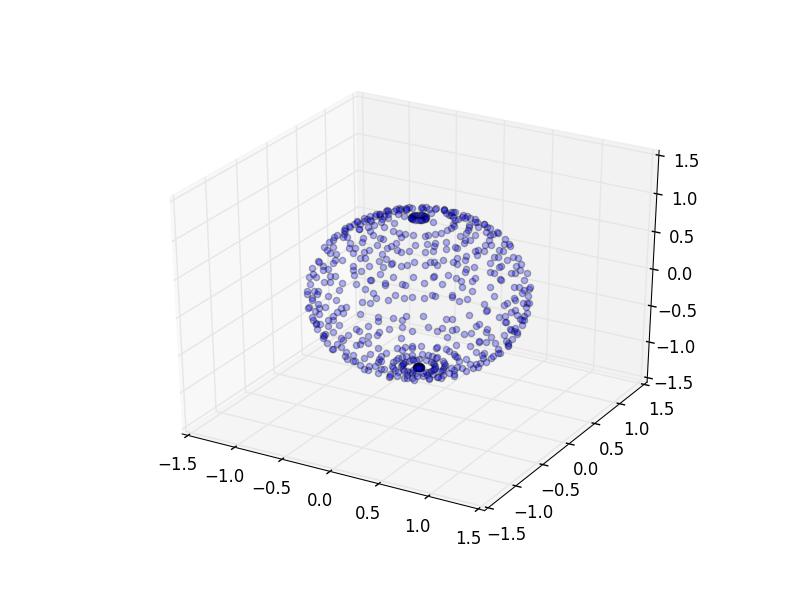
\includegraphics[width=\linewidth]{images/original_ellipsoid.png}
  \caption{Original ellipsoid}
\endminipage\hfill
\minipage{0.32\textwidth}
  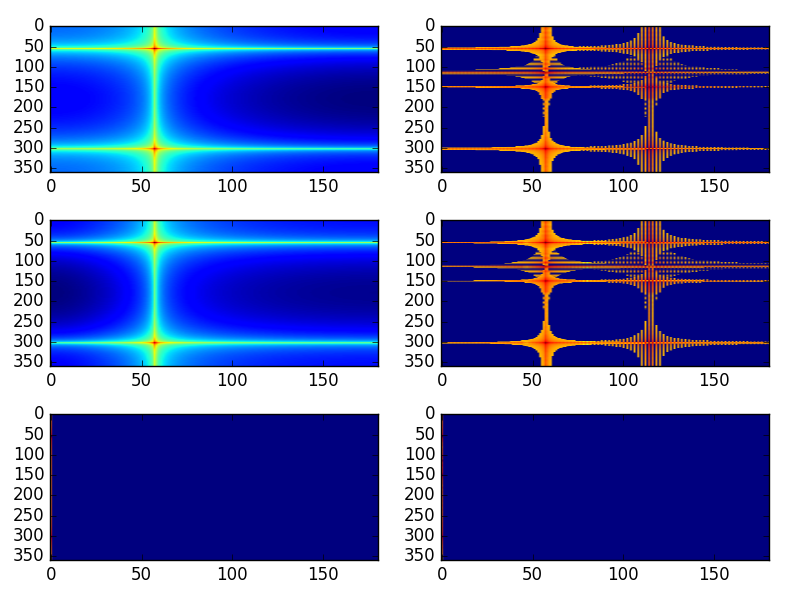
\includegraphics[width=\linewidth]{images/spectra_adjusted2.png}
  \caption{Left: original spectra, right: adjusted spectra}
\endminipage\hfill
\minipage{0.32\textwidth}%
  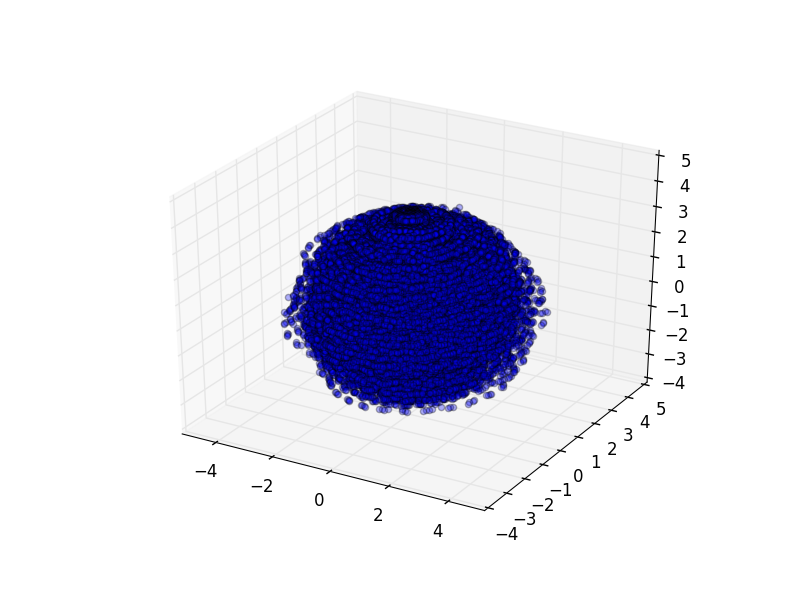
\includegraphics[width=\linewidth]{images/ellipsoid_backtransformed3.png}
  \caption{Ellipsoid backtransformed}
\endminipage
\end{figure}